\chapter{Il Teorema di Mozzi}
Se in un moto di un corpo rigido poniamo
\[
\underline{\omega}=\text{cost.}
\]
allora esiste unico un asse di rotazione fisso. Possiamo avere due casi:

\begin{itemize}
    \item[(i)] i punti $q$ lungo l'asse di rotazione sono fermi
    \[
    \underline{v}_q=0
    \]
    e allora
    \[
    \underline{v}_p=\underline{\omega}\wedge(\underline{x}_p-\underline{x}_q).
    \]
    I punti del corpo rigido descrivono nello spazio traiettorie circolari di raggio uguale alla distanza di $\underline{x}_p$ dall'asse di rotazione.

    \item[(ii)] punti $\underline{x}_q$ lungo l'asse con velocità parallela all'asse.

    La traiettoria di $\underline{x}_p$ è un'elica; se $\underline{v}_q$ è costante l'elica è di passo fissato, altrimenti ha passo variabile.
\end{itemize}

\begin{lemma}{}
Dati due vettori $\underline{a} \ne \underline{0},\underline{b} \in \mathbb{R}^3$, se $\underline{a}\cdot \underline{b} = 0$ allora la relazione
\[
\underline{a}\wedge \underline{x}=\underline{b}
\]
individua una retta.
\end{lemma}
\begin{proof}
Fissiamo
\[
\underline{a}=(a_1,a_2,a_3)\in\mathbb{R}^3.
\]
Consideriamo l'applicazione lineare
\[
L:\mathbb{R}^3\to\mathbb{R}^3,
\qquad
\underline{x}\longmapsto \underline{a}\wedge \underline{x}.
\]

Rappresentiamo $L$ tramite una matrice $A\in\mathbb{R}^{3,3}$ attraverso la base canonica in partenza e in arrivo.
\[
A=\bigl([L(e_1)]_{\mathcal E},\ [L(e_2)]_{\mathcal E},\ [L(e_3)]_{\mathcal E}\bigr)
\]

\[
L(e_1)=
\begin{pmatrix}
a_1\\
a_2\\
a_3
\end{pmatrix}
\wedge
\begin{pmatrix}
1\\
0\\
0
\end{pmatrix}
=
\begin{vmatrix}
\hat{\imath} & \hat{\jmath} & \hat{k}\\
a_1 & a_2 & a_3\\
1 & 0 & 0
\end{vmatrix}
=
\hat{\jmath}(a_3)-\hat{k}(a_2)
=
\begin{pmatrix}
0\\
a_3\\
-a_2
\end{pmatrix}
\]

\[
L(e_2)=
\begin{pmatrix}
a_1\\
a_2\\
a_3
\end{pmatrix}
\wedge
\begin{pmatrix}
0\\
1\\
0
\end{pmatrix}
=
\begin{vmatrix}
\hat{\imath} & \hat{\jmath} & \hat{k}\\
a_1 & a_2 & a_3\\
0 & 1 & 0
\end{vmatrix}
=
-a_3\hat{\imath}+a_1\hat{k}
=
\begin{pmatrix}
-a_3\\
0\\
a_1
\end{pmatrix}
\]

\[
L(e_3)=
\begin{pmatrix}
a_1\\
a_2\\
a_3
\end{pmatrix}
\wedge
\begin{pmatrix}
0\\
0\\
1
\end{pmatrix}
=
\begin{vmatrix}
\hat{\imath} & \hat{\jmath} & \hat{k}\\
a_1 & a_2 & a_3\\
0 & 0 & 1
\end{vmatrix}
=
a_2\hat{\imath}-a_1\hat{\jmath}
=
\begin{pmatrix}
a_2\\
-a_1\\
0
\end{pmatrix}
\]

\[
\Rightarrow\quad
A=
\begin{pmatrix}
0 & -a_3 & a_2\\
a_3 & 0 & -a_1\\
-a_2 & a_1 & 0
\end{pmatrix}
\]

$L$ è quindi rappresentata da una matrice antisimmetrica ovvero
\[
A^T=-A
\iff
A=-A^T
\]

\[
\Rightarrow\quad
\det(A)=\det(A^T)=\det(-A^T)=-\det(A)
\iff
\det(A)=0
\]

Abbiamo quindi ottenuto che $L_A$ (e quindi $L$) non è una mappa iniettiva. Di conseguenza il nucleo di $L_A$ ha dimensione maggiore o uguale a $1$. Il caso
\[
\dim(\ker L_A)=3
\]
è assurdo perché implica
\[
\operatorname{Im}(L_A)=\{0\}
\]
ovvero
\[
\underline{a}=0.
\]
Il caso
\[
\dim(\ker L_A)=2
\]
è altrettanto problematico perché implica che
\[
\dim(\operatorname{Im}(L_A))=1
\]
ovvero che tutti i prodotti vettoriali di $\underline{a}$ con $\underline{x}\in\mathbb{R}^3$ stanno su una retta. Limitiamoci a
\[
\dim(\ker L_A)=1.
\]
Allora se
\[
\underline{b}\in\operatorname{Im}(L_A)
\]
le soluzioni di
\[
A\underline{x}=\underline{b}
\]
sono quindi un affine di $\ker(L_A)$ e quindi una retta.\\
Notiamo che per costruzione del prodotto vettoriale $\operatorname{Ker}(L) = \operatorname{span}(\underline{a})$ ovvero la  retta trovata è affine e con vettore direttore $\underline{a}$.\\
Notiamo infine che se $\underline{a} \ne \underline{0}$ allora
\[
\underline{b} \in \operatorname{Im}(L_A) \Leftrightarrow \underline{a} \cdot \underline{b} = 0
\]
per le proprietà del prodotto vettoriale
\end{proof}
\begin{oss}{}
Per trovare la retta individuata da
\[
\underline{a}\wedge \underline{x}=\underline{b}
\qquad \text{con } \underline{a}\neq \underline{0}
\quad \text{e} \quad
\underline{a}\cdot \underline{b}=0
\]
in forma parametrica possiamo procedere come segue.

Se
\[
L:\mathbb{R}^3\to\mathbb{R}^3,
\qquad
\underline{x}\mapsto \underline{a}\wedge \underline{x},
\]
allora
\[
L^{-1}(\{\underline{b}\})=\underline{x}_0+\ker(L)=\underline{x}_0+\mathrm{Span}\{\underline{a}\},
\qquad
\text{con } \underline{x}_0\in L^{-1}(\{\underline{b}\}).
\]

Per concludere basta notare che
\[
\underline{x}_0=-\frac{\underline{a}\wedge \underline{b}}{\|\underline{a}\|^2}
\]
fa al caso nostro. Infatti
\[
L\left(-\frac{\underline{a}\wedge \underline{b}}{\|\underline{a}\|^2}\right)
=
-\frac{1}{\|\underline{a}\|^2}\Bigl(\underline{a}\wedge(\underline{a}\wedge \underline{b})\Bigr)
=
-\frac{1}{\|\underline{a}\|^2}\Bigl(\underline{a}\,(\underline{a}\cdot \underline{b})-\underline{b}\,(\underline{a}\cdot \underline{a})\Bigr)
=
-\frac{1}{\|\underline{a}\|^2}\cdot\bigl(-\underline{b}\,\|\underline{a}\|^2\bigr)
=
\underline{b}.
\]

Dunque la retta si scrive in forma parametrica come
\[
\underline{x}_t=t\,\underline{a}-\frac{\underline{a}\wedge \underline{b}}{\|\underline{a}\|^2},
\qquad
t\in\mathbb{R}.
\]

\end{oss}

\begin{theorem}{}[di Mozzi]
    La traiettoria di un punto di un corpo rigido che si muove di un moto qualsiasi è istantaneamente elicoidale.
\end{theorem}
\begin{proof}
Per ogni moto possiamo scrivere
\[
\underline{v}_p=\underline{v}_q+\underline{\omega}\wedge(\underline{x}_p-\underline{x}_q)
\]

Decomponiamo lungo la direzione parallela e perpendicolare a $\underline{\omega}$
\[
\underline{v}_q=\underline{v}_q^{\parallel}+\underline{v}_q^{\perp}
\]

\[
\underline{v}_q^{\parallel}
=
\left(
\underline{v}_q\cdot
\left(
\frac{\underline{\omega}}{\|\underline{\omega}\|}
\right)
\right)
\frac{\underline{\omega}}{\|\underline{\omega}\|}
\]

\[
\underline{v}_q^{\perp}=\underline{v}_q-\underline{v}_q^{\parallel}
\]

L'idea è quella di riuscire a far vedere che il moto del generico punto $\underline{x}_q$ o $\underline{x}_p$ è composto da una velocità parallela all'asse di rotazione più una velocità perpendicolare all'asse che produca un moto circolare attorno l'asse stesso. Un punto dell'asse  $\underline{x}_r$ deve quindi soddisfare la seguente condizione che impone proprio la velocità di un moto circolare attorno all'asse.
\[
\underline{v}_q^{\perp}
=
\underline{\omega}\wedge(\underline{x}_q-\underline{x}_r)
\iff
\underline{\omega}\wedge \underline{x}_r
=
-\underline{v}_q^{\perp}
+
\underline{\omega}\wedge \underline{x}_q
\]

Per il lemma gli $\underline{x}_r$ individuano una retta affine di direzione $\underline{\omega}$. Sostituisco
\[
\underline{v}_q^{\perp}
=
\underline{\omega}\wedge(\underline{x}_q-\underline{x}_r)
\]
in
\[
\underline{v}_p=\underline{v}_q^{\parallel}+\underline{v}_q^{\perp}+\underline{\omega}\wedge(\underline{x}_p-\underline{x}_q)
\]

\[
\underline{v}_p
=
\underline{v}_q^{\parallel}
+
\underline{\omega}\wedge(\underline{x}_q-\underline{x}_r)
+
\underline{\omega}\wedge(\underline{x}_p-\underline{x}_q)
=
\]

\[
=
\underline{v}_q^{\parallel}
+
\underline{\omega}\wedge(\underline{x}_p-\underline{x}_r)
\]

Il moto trovato è un moto elicoidale e l'insieme dei punti $\{\underline{x}_r\}$ è detto asse di Mozzi.
\end{proof}
\begin{oss}{}
    $\underline{x_r}$ non è necessariamente un punto del corpo.
\end{oss}
\begin{oss}{}
La velocità $\underline{v}_{q}^{\parallel}$ usata a fine dimostrazione in
\[
\underline{v}_{p}=\underline{v}_{q}^{\parallel}+\underline{\omega}\wedge\left(\underline{x}_{p}-\underline{x}_{r}\right)
\]
è la velocità istantanea di ogni punto dell'asse. Infatti, se $\underline{x}_{p}=\underline{x}_{s}$ è un punto dell'asse, otteniamo
\[
\underline{v}_{s}=\underline{v}_{q}^{\parallel}+\underline{\omega}\wedge\left(\underline{x}_{s}-\underline{x}_{r}\right).
\]
E dal momento che
\[
\underline{x}_{s}-\underline{x}_{r}\parallel \underline{\omega}
\]
otteniamo
\[
\underline{v}_{s}=\underline{v}_{q}^{\parallel}.
\]

In particolare tutti i punti dell'asse di Mozzi hanno stessa velocità istantanea, che coincide con la proiezione della velocità di un qualsiasi punto $\underline{x}_{q}$ lungo l'asse.

\end{oss}
\begin{oss}{}
    La descrizione del moto non dipende dal punto dell'asse scelto. Infatti se $\underline{x_{r_1}}$ e $\underline{x_{r_2}}$ sono due punti dell'asse parallelo a $\underline{\omega}$ e $\underline{x_p}$ è un punto qualsiasi si ha che
    \[
        \underline{\omega} \wedge (\underline{x_p} - \underline{x_{r_1}}) =  \underline{\omega} \wedge (\underline{x_p} - \underline{x_{r_2}})
    \]

    \begin{center}
\begin{tikzpicture}[scale=1.1]
    % asse
    \draw[line width=0.9pt] (-4.2,0) -- (4.8,0);
    \node[right] at (4.9,0) {ASSE};

    % punti sull'asse
    \coordinate (R1) at (-1.6,0);
    \coordinate (R2) at (1.8,0);
    \coordinate (M) at (0,0);
    \coordinate (P) at (0,2.0);

    \fill[red] (R1) circle (2pt);
    \fill[red] (R2) circle (2pt);
    \fill (M) circle (2pt);
    \fill (P) circle (2pt);

    % segmenti
    \draw[line width=0.9pt] (R1) -- (P);
    \draw[line width=0.9pt] (R2) -- (P);
    \draw[dashed] (M) -- (P);

    % etichette punti
    \node[below] at (R1) {$\underline{x}_{r_1}$};
    \node[below] at (R2) {$\underline{x}_{r_2}$};
    \node[above] at (P) {$\underline{x}_p$};

    % etichette segmenti
    \node[above left] at (-0.9,1.25) {$\underline{x}_p-\underline{x}_{r_1}$};
    \node[above right] at (1.0,1.25) {$\underline{x}_p-\underline{x}_{r_2}$};

    % distanza d
    \node[right] at (0.05,1.0) {$d$};

    % frecce w/|w|
    \draw[red,->,line width=0.9pt] (-1.6,0) -- (-0.55,0);
    \draw[red,->,line width=0.9pt] (1.8,0) -- (2.85,0);
    \node[red,below] at (-1.08,-0.05) {$\dfrac{\underline{\omega}}{\|\underline{\omega}\|}$};
    \node[red,below] at (2.33,-0.05) {$\dfrac{\underline{\omega}}{\|\underline{\omega}\|}$};

    % angoli
    \draw[->] (-1.15,0) arc[start angle=0,end angle=50,radius=0.45];
    \node at (-1.0,0.32) {$\theta$};

    \draw[->] (1.35,0) arc[start angle=180,end angle=130,radius=0.45];
    \node at (0.8,0.24) {$\pi - \varphi$};
\end{tikzpicture}
\end{center}

Infatti, calcolando la differenza tra i due termini si ottiene:
\[
\underline{\omega}\wedge(\underline{x}_p-\underline{x}_{r_1}) - \underline{\omega}\wedge(\underline{x}_p-\underline{x}_{r_2}) = \underline{\omega}\wedge(\underline{x}_{r_2}-\underline{x}_{r_1}) = \underline{0}
\]
poiché $\underline{x}_{r_1}$ e $\underline{x}_{r_2}$ appartengono allo stesso asse, il vettore $(\underline{x}_{r_2}-\underline{x}_{r_1})$ è parallelo a $\underline{\omega}$. Di conseguenza, i due prodotti vettoriali sono identici.
\end{oss}


\begin{oss}{}
    Possiamo ricavare i punti dell'asse in forma parametrica tramite
\[
\underline{\omega}\wedge \underline{x}_r
=
-\underline{v}_q^{\perp}+\underline{\omega}\wedge \underline{x}_q
\qquad \Rightarrow \qquad
\underline{x}_r
=
t\,\underline{\omega}
-
\frac{\underline{\omega}\wedge\left(-\underline{v}_q^{\perp}+\underline{\omega}\wedge \underline{x}_q\right)}{\|\underline{\omega}\|^2},
\qquad t\in\mathbb{R}.
\]

Oppure in forma cartesiana utilizzando il fatto che
\[
\underline{v}_r \parallel \underline{\omega}
\qquad \forall\,\underline{x}_r
\text{ appartenente all'asse}
\]
tramite
\[
\frac{v_r^x}{\omega_x}
=
\frac{v_r^y}{\omega_y}
=
\frac{v_r^z}{\omega_z}.
\]

Dove $v_r^x$, $v_r^y$, $v_r^z$ devono essere espresse in funzione di
$x_r$, $y_r$, $z_r$, ad esempio utilizzando la formula fondamentale della cinematica.
\end{oss}

\begin{oss}{}
Nel caso di moti piani
\[
\underline{\omega}=(0,0,\omega_z)
\]
l'asse di Mozzi è ortogonale al piano del moto e ha un punto sul piano del moto. Intorno a questo punto $\bar{q}$, detto centro di istantanea rotazione, il moto è istantaneamente solo rotazionale:
\[
\underline{v}_p=\underline{\omega}\wedge(\underline{x}_p-\underline{x}_{\bar{q}}).
\]
Questo infatti è soggetto al vincolo $z_{\overline{q}} = 0 \Rightarrow \underline{v}_{\overline{q}} = 0$ essendo tutta la velocità di $\overline{q}$ diretta lungo l'asse $z$.
\end{oss}
\begin{example}{}
    Vogliamo studiare la posizione dell'asse di Mozzi di una trottola. Supponiamo che
la trottola sia a regime e che quindi abbia velocità angolare perpendicolare
al piano. Possiamo quindi studiare il moto come moto piano e cercare il centro
di istantanea rotazione.

\begin{figure}
\centering
\begin{minipage}{0.34\textwidth}
\centering
\begin{tikzpicture}[scale=1.2]
  % assi
  \draw[->] (0,0) -- (2.2,0) node[right] {$u$};
  \draw[->] (0,0) -- (0,2.2) node[above] {$z$};
  \draw[->] (0,0) -- (-1.3,-1.3) node[below] {$x$};

  % trottola
  \draw (-0.5,0.95) .. controls (-0.25,1.15) and (0.25,1.15) .. (0.5,0.95);
  \draw (-0.5,0.95) .. controls (-0.2,0.72) and (0.2,0.72) .. (0.5,0.95);
  \draw (-0.5,0.95) -- (-0.2,0.25);
  \draw (0.5,0.95) -- (0.2,0.25);
  \draw (-0.2,0.25) -- (0.2,0.25);
  \draw (-0.2,0.25) -- (0,-0.45);
  \draw (0.2,0.25) -- (0,-0.45);
  \fill (0,-0.45) circle (1.2pt);
  \node[below right] at (0,-0.45) {$c$};

  % omega
  \draw[red,->,line width=0.9pt] (0.25,1.05) -- (0.25,2.0);
  \node[red,right] at (0.25,1.65) {$\omega$};
\end{tikzpicture}
\end{minipage}
\hfill
\begin{minipage}{0.48\textwidth}
\centering
\begin{tikzpicture}[scale=1.2]
  % assi
  \draw[->] (-0.2,0) -- (3.2,0) node[right] {$x$};
  \draw[->] (0,-1.2) -- (0,2.2) node[above] {$u$};

  % disco
  \draw (1.45,1.25) circle (0.65);
  \fill (1.45,1.25) circle (1.1pt);
  \node[below right] at (1.45,1.25) {$c$};

  % velocità
  \draw[->,line width=0.9pt] (1.45,1.25) -- (1.1,1.72);
  \node[above left] at (1.23,1.55) {$\underline{v}_c$};

  % omega
  \draw[red,->,line width=0.9pt] (2.02,2.02) arc[start angle=20,end angle=160,radius=0.63];
  \node[red] at (1.45,2.25) {$\omega$};
\end{tikzpicture}
\end{minipage}
\end{figure}

Sia $\underline{x}_I$ il centro di istantanea rotazione. Sappiamo che
$\underline{v}_I=\underline{v}_p^{\parallel}=0 \ \forall p$. Allora
\[
0=\underline{v}_c+\omega\wedge(\underline{x}_I-\underline{x}_c)
\]
\[
\Rightarrow\quad
0=\hat{k}\wedge \underline{v}_c+\hat{k}\wedge\bigl(\omega\wedge(\underline{x}_I-\underline{x}_c)\bigr)
\]
\[
\Rightarrow\quad
0=\hat{k}\wedge \underline{v}_c+\omega\cdot \|\underline{x}_I-\underline{x}_c\|\cdot
\hat{k}\wedge\left(\hat{k}\wedge
\frac{\underline{x}_I-\underline{x}_c}{\|\underline{x}_I-\underline{x}_c\|}\right)
\]
ora dal momento che $ \frac{\underline{x}_I-\underline{x}_c}{\|\underline{x}_I-\underline{x}_c\|}$ ha coordinata lungo $\hat k$ nulla risulta che
\[
\Rightarrow\quad
0=\hat{k}\wedge \underline{v}_c-\omega\cdot \|\underline{x}_I-\underline{x}_c\|\cdot
\frac{\underline{x}_I-\underline{x}_c}{\|\underline{x}_I-\underline{x}_c\|}
=
\hat{k}\wedge \underline{v}_c-\omega\cdot(\underline{x}_I-\underline{x}_c)
\]
\[
\Rightarrow\quad
\underline{x}_I-\underline{x}_c=\frac{\hat{k}\wedge \underline{v}_c}{\omega}
\qquad \Rightarrow \qquad
\underline{x}_I=\underline{x}_c+\frac{\hat{k}\wedge \underline{v}_c}{\omega}.
\]

Abbiamo quindi ottenuto che $\underline{x}_I$ sta sulla retta perpendicolare a
$\underline{v}_c$ e passante per $\underline{x}_c$. Il verso dipende dal segno di $\omega$.

\begin{figure}
\centering
\begin{tikzpicture}[scale=1.25]
  % assi
  \draw[->] (-0.2,0) -- (3.2,0) node[right] {$x$};
  \draw[->] (0,-1.4) -- (0,2.2) node[above] {$u$};

  % retta tratteggiata
  \draw[dashed] (-0.625 , -0.6) -- (2.5,2.4);

  % disco
  \draw (1.25,1.2) circle (0.62);
  \fill (1.25,1.2) circle (1.1pt);
  \node[below right] at (1.25,1.2) {$c$};

  % velocità
  \draw[->,line width=0.9pt] (1.25,1.2) -- (0.92,1.64);
  \node[above left] at (1.06,1.48) {$\underline{v}_c$};

  % omega
  \draw[red,->,line width=0.9pt] (1.8,1.95) arc[start angle=20,end angle=160,radius=0.6];
  \node[red] at (1.24,2.18) {$\omega$};

  % x_I
  \coordinate (XI) at (0.625,0.6);
  \draw[green!60!black,->,line width=1pt] (0,0) -- (XI);
  \fill[green!60!black] (XI) circle (1.2pt);
  \node[green!60!black,above left] at (XI) {$\underline{x}_I$};
\end{tikzpicture}
\end{figure}

Più nello specifico la distanza dal centro $c$ vale
\[
\|\underline{x}_I-\underline{x}_c\|
=
\left\|\frac{\hat{k}\wedge \underline{v}_c}{\omega}\right\|
=
\frac{\|\hat{k}\wedge \underline{v}_c\|}{|\omega|}
=
\frac{\|\underline{v}_c\|}{|\omega|}
\qquad
(\hat{k}\perp \underline{v}_c).
\]

E quindi nel caso in cui $\underline{v}_c=0$ l'asse di Mozzi coincide con
l'asse verticale di simmetria della trottola.

In generale il centro di istantanea rotazione può essere un punto interno
alla trottola, sul bordo o esterno.
\end{example}
\begin{examplebreak}{}
    Troviamo il centro di istantanea rotazione del sistema caratterizzato dai vincoli $x_A = y_B = 0$ che ha quindi un solo grado di libertà.
\begin{center}
\begin{tikzpicture}[scale=1.15]
    % assi
    \draw[->] (-0.6,0) -- (5.2,0);
    \draw[->] (0,-0.6) -- (0,3.6);

    % punti
    \coordinate (A) at (0,2.7);
    \coordinate (B) at (4.0,0);
    \coordinate (Q) at (4.0,2.7);

    % asta
    \draw[line width=0.9pt] (A) -- (B);
    \node at (2.15,1.65) {$\ell$};

    % tratteggi
    \draw[dashed] (A) -- (Q);
    \draw[dashed] (B) -- (Q);

    % punti marcati
    \fill (A) circle (1.8pt);
    \fill (B) circle (1.8pt);
    \fill (Q) circle (1.8pt);

    % etichette
    \node[left] at (A) {$\underline{x}_A$};
    \node[below] at (B) {$\underline{x}_B$};
    \node[above] at (Q) {$\underline{x}_q$};

    % velocità
    \draw[->,red,line width=0.9pt] (A) -- ++(0,-1.0);
    \node[red,left] at (-0.05,1.75) {$\underline{v}_A$};

    \draw[->,red,line width=0.9pt] (B) -- ++(1.0,0);
    \node[red,above] at (4.55,0.05) {$\underline{v}_B$};
\end{tikzpicture}
\end{center}



\[
\underline{v}_A=\underline{\omega}\wedge(\underline{x}_A-\underline{x}_q)
\qquad\Rightarrow\qquad
\underline{x}_A-\underline{x}_q \text{ è parallelo a } \hat{\imath}
\]

\[
\underline{v}_B=\underline{\omega}\wedge(\underline{x}_B-\underline{x}_q)
\qquad\Rightarrow\qquad
\underline{x}_B-\underline{x}_q \text{ è parallelo a } \hat{\jmath}
\]

In particolare
\[
\underline{x}_A-\underline{x}_q\in \operatorname{span}\{\hat{\imath}\}
\qquad\text{e}\qquad
\underline{x}_B-\underline{x}_q\in \operatorname{span}\{\hat{\jmath}\}.
\]

Ovvero
\[
\underline{x}_q\in \underline{x}_A+\operatorname{span}\{\hat{\imath}\},
\qquad
\underline{x}_q\in \underline{x}_B+\operatorname{span}\{\hat{\jmath}\},
\]
ovvero
\[
\underline{x}_q\in
\bigl(\underline{x}_A+\operatorname{span}\{\hat{\imath}\}\bigr)
\cap
\bigl(\underline{x}_B+\operatorname{span}\{\hat{\jmath}\}\bigr).
\]

Ma dal momento che
\[
\operatorname{span}\{\hat{\jmath}\}\cap \operatorname{span}\{\hat{\imath}\}=\{0\},
\]
$\underline{x}_q$ è l'unico vettore nell'intersezione dei due affini e può essere individuato geometricamente come in figura o analiticamente dai vincoli
\[
y=y_A
\qquad\text{e}\qquad
x=x_B.
\]
\end{examplebreak}
